\chapter{Avaliação}
\label{cap:avaliacao}

Este capítulo apresenta a avaliação da solução implementada, tanto em termos funcionais como de desempenho. O objetivo é demonstrar a viabilidade da arquitetura proposta, analisando a sua usabilidade, a robustez dos mecanismos criptográficos edesempenho.

\section{Avaliação Funcional}

Para validar o correto funcionamento da solução, foram realizados testes que cobrem o fluxo completo de consentimento:

\begin{enumerate}
    \item Apresentação do \textit{banner} de consentimento através do Klaro.js.
    \item Captura da interação do utilizador pela extensão no cliente.
    \item Assinatura digital do consentimento no cliente.
    \item Envio do consentimento assinado para o servidor.
    \item Validação da assinatura do cliente no servidor.
    \item Criação de um JWS com assinaturas do cliente e servidor.
    \item Validação final pelo cliente e registo local do consentimento.
\end{enumerate}

A Figura~\ref{fig:klarojs-banner} já ilustrou a interface do banner apresentada ao utilizador.  
De seguida, mostram-se exemplos de payloads e respetivos JWS gerados pelo sistema.

\begin{figure}[h]
    \centering
	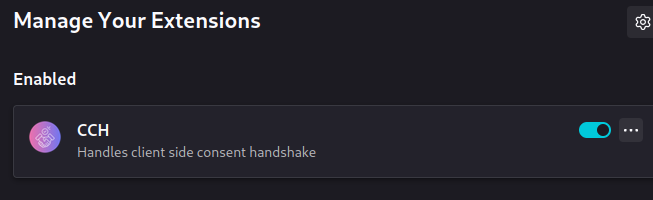
\includegraphics[width=0.8\textwidth]{images/cch.png}
    \caption{Extensão carregada no browser}
    %\label{fig:cch}
\end{figure}

\newpage

\textbf{Exemplo 1 — Recusar todos os consentimentos}
\begin{lstlisting}[caption={Payload com rejeição de todos os consentimentos.}]
{
  consents: {
    twitter: false,
    youtube: false,
    matomo: false,
    inlineTracker: false,
    externalTracker: false,
    intercom: false,
    mouseflow: false,
    adsense: false,
    camera: false,
    cloudflare: true
  },
  confirmed: false,
  timestamp: '2025-10-01T17:14:47.863Z'
}
\end{lstlisting}

\begin{lstlisting}[ caption={Exemplo de JWS gerado para recusar todos os consentimentos.}]
{
    "payload":"eyJjb...",
    "signatures":[
        {
            "header":{"typ":"JWT","alg":"PS256"},"signature":"g_EO73..."
        },
        {
            "header":{"typ":"JWT","alg":"PS256"},"signature":"iLcMTs..."
        }
    ]
}
\end{lstlisting}

Podemos ver aqui as principais estruturas de dados que são trocadas entre o cliente e servidor.

\textbf{Exemplo 2 — Aceitar todos os consentimentos}
\begin{lstlisting}[ caption={Payload com aceitação de todos os consentimentos.}]
{
  consents: {
    twitter: true,
    youtube: true,
    matomo: true,
    inlineTracker: true,
    externalTracker: true,
    intercom: true,
    mouseflow: true,
    adsense: true,
    camera: true,
    cloudflare: true
  },
  confirmed: true,
  timestamp: '2025-10-01T17:15:33.744Z'
}
\end{lstlisting}

\begin{lstlisting}[caption={Exemplo de JWS gerado para aceitação de todos os consentimentos.}]
{
    "payload":"eyJjb...",
    "signatures":[
        {
            "header":{"typ":"JWT","alg":"PS256"},
            "signature":"n0VOK..."
        },
        {
            "header":{"typ":"JWT","alg":"PS256"},"signature":"f2lBlY..."
        }
    ]
}
\end{lstlisting}

No caso da aceitação dos consentimentos, a funcionalidade e a estrutura dos dados não se altera significativamente.

\textbf{Exemplo 3 — Subconjunto de consentimentos (5 serviços)}

Foram também realizados testes com \textit{payloads} reduzidos, contendo apenas 5 serviços. Os resultados confirmam que, consoante for menor o \textit{payload}, melhor são os tempos de verificação e criação dos JWS.

\section{Avaliação de Desempenho}

Foram conduzidos testes de medições de desempenho para avaliar a eficiência da solução. Os tempos de execução foram registados, tanto para a criação do JWS, como para a verificação da assinatura. A Tabela~\ref{tab:performance} resume os resultados obtidos.
É necessário ter em conta que, na própria criação do JWS é feita ainda a assinatura do servidor sobre o consentimento. E a verificação da assinatura do cliente é efetuada pelo servidor.

\begin{table}[h]
    \centering
    \caption{Resultados de desempenho em diferentes cenários de payload.}
    \label{tab:performance}
    \begin{tabular}{|c|c|c|c|}
        \hline
        \textbf{Cenário} & \textbf{Tamanho do payload} & \textbf{Tempo verificação} & \textbf{Tempo criação JWS} \\ \hline
        Recusa total   & 248 bytes & 1.003 ms & 6.172 ms \\ \hline
        Aceitação total & 238 bytes & 1.084 ms & 6.542 ms \\ \hline
        Recusa (5 serviços) & 155 bytes & 0.532 ms & 2.952 ms \\ \hline
        Aceitação (5 serviços) & 150 bytes & 0.416 ms & 2.267 ms \\ \hline
    \end{tabular}
\end{table}

Estes resultados demonstram que, tanto a criação do JWS, como a verificação das assinaturas digitais, apresentam tempos de execução reduzidos. No entanto, estes valores têm alguma variedade, mas podemos ver como a diferença do tamanho do \textit{payload} provoca a diferença entre os tempos de criação do JWS e verificação da assinatura.

\section{Discussão dos Resultados}

A análise dos resultados permite constatar que o fluxo funcional de consentimento foi corretamente validado em vários cenários, desde a recusa total até à aceitação de todos os serviços, passando também por subconjuntos de consentimentos. Em todos os casos, a criação e validação de JWS foi executada com sucesso, confirmando a robustez da solução implementada.

No que respeita ao desempenho, verificou-se que o impacto do tamanho do \textit{payload} nos tempos de execução é significativo. Embora exista uma variação ligeira e proporcional entre os cenários de menor e maior dimensão, os valores registados mantêm-se sempre baixos, tanto para a criação de JWS como para a sua verificação no servidor.

Em termos práticos, estes resultados demonstram que a solução consegue cumprir os objetivos estabelecidos: assegurar a transparência e a auditabilidade dos consentimentos digitais através do registo JWS, preservando simultaneamente a integridade e a autenticidade das assinaturas, sem comprometer a experiência de utilização ou a escalabilidade do sistema.
